\section{Introduction}

% A few sentences placing the work in high-level context. Limit it to a few paragraphs at most; your report is on reproducing a piece of work, you don’t have to motivate that work.

The original paper discusses a new non-autoregressive language model called Diffusion-LM, which is based on continuous diffusions. Diffusion-LM iteratively denoises a sequence of Gaussian vectors into word vectors to produce a sequence of intermediate latent variables. The continuous, hierarchical nature of these intermediate variables enables a simple gradient-based algorithm to perform complex, controllable generation tasks. The authors demonstrate successful control of Diffusion-LM for six challenging fine-grained control tasks, outperforming prior work.

\section{Scope of reproducibility}
\label{sec:claims}

% Introduce the specific setting or problem addressed in this work, and list the main claims from the original paper. Think of this as writing out the main contributions of the original paper. Each claim should be relatively concise; some papers may not clearly list their claims, and one must formulate them in terms of the presented experiments. (For those familiar, these claims are roughly the scientific hypotheses evaluated in the original work.)

% A claim should be something that can be supported or rejected by your data. An example is, ``Finetuning pretrained BERT on dataset X will have higher accuracy than an LSTM trained with GloVe embeddings.''
% This is concise, and is something that can be supported by experiments.
% An example of a claim that is too vague, which can't be supported by experiments, is ``Contextual embedding models have shown strong performance on a number of tasks. We will run experiments evaluating two types of contextual embedding models on datasets X, Y, and Z."

The central claim of the paper is that a language model trained via a continuous diffusion process learns hierarchical representations, and that constraints can be placed in this latent space that allow for richer controls than those from autoregressive language models which can only condition text on the left context.

To this aim, the following control experiments are considered in the original paper:

% Each experiment in Section~\ref{sec:results} will support (at least) one of these claims, so a reader of your report should be able to separately understand the \emph{claims} and the \emph{evidence} that supports them.

\begin{itemize}
\item \textbf{Semantic Content}: Given a field and value, generate a sentence that covers the field and value, and report the success rate by exact match of the value.
\item \textbf{Parts-of-speech}: Given a sequence of parts-of-speech tags, generate a sequence of words whose POS tags match the target. Success is measured via word-level exact match.
\item \textbf{Syntax Tree}: Given a target syntactic parse tree, generate text whose syntactic parse matches the given parse. Success is evaluated using F1 scores.
\item \textbf{Syntax Spans}: Given a target pair of span and syntactic category, generate text whose parse tree over the span matches the target syntactic category. Success is measured by the fraction of spans that match exactly.
\item \textbf{Length}: Given a target length, generate a sequence with a length within ±2 of the target.
\item \textbf{Infilling}: Given left and right contexts, generate a sentence that logically connects the two. Both automatic and human evaluation is used for evaluation.
\end{itemize}

Therefore, a faithful reproduction of the original work would involve rerunning these experiments and calculating their results.

%\jdcomment{To organizers: I asked my students to connect the main claims and the experiments that supported them. For example, in this list above they could have ``Claim 1, which is supported by Experiment 1 in Figure 1.'' The benefit was that this caused the students to think about what their experiments were showing (as opposed to blindly rerunning each experiment and not considering how it fit into the overall story), but honestly it seemed hard for the students to understand what I was asking for.}

\section{Related work}
% The paper you are reproducing already has related works. Rather than just copying, focus on the relevant papers they cited (you may ignore non-relevant related works) from the perspective of the challenge. You should also include papers that were not cited by the work you are reproducing (for example, works published after/concurrently, or that were simply missed by your paper).

\section{Methodology}

% Explain your approach - did you use the author's code, or did you aim to re-implement the approach from the description in the paper? Summarize the resources (code, documentation, GPUs) that you used.

For the reproduction of the results in the paper, I primarily relied on the author's source code. While I initially attempted to write my own implementation, I was unable to do so within the time constraints. However, I was able to uncover some details of the authors' implementation that were not mentioned in the paper.

My experiments were run using a single NVIDIA A100 GPU to retrain the E2E dataset model in under 10 hours. For the larger ROC stories dataset, I used 16 NVIDIA Quadro RTX 8000 GPUs to train the model in under 20 hours. I then used the models I trained to implement the control tests described in the paper.

\subsection{Model descriptions}

Diffusion-LM is a diffusion model that involves iterative denoising of a Gaussian noise signal. During training, the text is converted into tokens by means of a default BERT tokenizer. These tokens are then embedded into a low-dimensional (e.g. $d=16$) latent space and upsampled by a fully connected network to match a Transformer encoder architecture.

As shown in Figure \ref{fig:graphical-model}, the token embeddings are iteratively noised according to a schedule parametrized by $q(x_t | x_{t-1}) = \mathcal{N}(x_t; \sqrt{1-\beta_t x_{t-1}}, \beta_t \mathbb{I})$. The $\beta_t$ values are chosen according to a scheduling function such that, after $T=2000$ steps, the resulting embeddings are normally distributed. This forward noise is then reversed by a Transformer model described by the Markov chain: $p_\theta(x_{t-1}|x_t) = \mathcal{N}(x_{t-1}; \mu_\theta(x_t, t), \Sigma_\theta (x_t, t))$.

The noised embeddings are then projected down to $d$ dimensions to match the input embedding size using another fully connected network. This noise removal process is applied to each sample from $x_T$ to $x_0$. A ``rounding step'' $p_\theta (w|x_0)$ is then used to map the resulting embeddings onto the nearest neighboring token using a softmax function.

\begin{figure}[h]
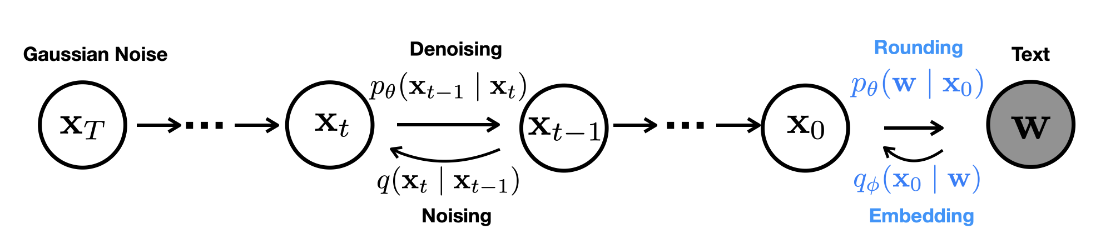
\includegraphics[scale=0.3]{images/diffusion-lm-graphical-model.png}
\centering
\caption{A graphical model representing the forward and reverse diffusion processes. In addition a rounding and embedding mapping is added to shift between continuous latents and the discrete token space.}
\label{fig:graphical-model}
\end{figure}

During training, a clamping trick is employed in which the denoised embeddings are clamped onto the nearest token exactly. This improved the model's stability during training, according to the authors.

The paper considered many different modifications to the diffusion process used during training, exploring hyperparameters such as the latent embedding dimension and different noise schedules. They also employed an analytical simplification of the variational lower bound loss function derived from the widely known image diffusion context.

In my work, I focused on the version from which I believe they derived their main results. The Diffusion-LM I considered is based on a Transformer architecture with 80M parameters which is basically the base bert uncased model from HuggingFace with default parameters. The input and output projection layers employed a single hidden layer of 768 dimensions (matching the embedding dimension of the BERT base model), and a tanh activation function.

\subsection{Datasets}

The authors trained Diffusion-LM on two datasets, E2E and ROCStories. The E2E dataset consists of 50K restaurant reviews labelled by 8 fields including food type, price and customer rating. The ROCStories dataset consists of 98K five-sentence stories, capturing a rich set of causal and temporal commonsense relations between daily events.



For each dataset include 1) relevant statistics such as the number of examples and label distributions, 2) details of train / dev / test splits, 3) an explanation of any preprocessing done, and 4) a link to download the data (if available).

\subsection{Hyperparameters}
Describe how the hyperparameter values were set. If there was a hyperparameter search done, be sure to include the range of hyperparameters searched over, the method used to search (e.g. manual search, random search, Bayesian optimization, etc.), and the best hyperparameters found. Include the number of total experiments (e.g. hyperparameter trials). You can also include all results from that search (not just the best-found results).

\subsection{Experimental setup and code}
Include a description of how the experiments were set up that's clear enough a reader could replicate the setup. 
Include a description of the specific measure used to evaluate the experiments (e.g. accuracy, precision@K, BLEU score, etc.). 
Provide a link to your code.

\subsection{Computational requirements}
Include a description of the hardware used, such as the GPU or CPU the experiments were run on. 
For each model, include a measure of the average runtime (e.g. average time to predict labels for a given validation set with a particular batch size).
For each experiment, include the total computational requirements (e.g. the total GPU hours spent).
(Note: you'll likely have to record this as you run your experiments, so it's better to think about it ahead of time). Generally, consider the perspective of a reader who wants to use the approach described in the paper --- list what they would find useful.

\section{Results}
\label{sec:results}
Start with a high-level overview of your results. Do your results support the main claims of the original paper? Keep this section as factual and precise as possible, reserve your judgement and discussion points for the next "Discussion" section. 


\subsection{Results reproducing original paper}
For each experiment, say 1) which claim in Section~\ref{sec:claims} it supports, and 2) if it successfully reproduced the associated experiment in the original paper. 
For example, an experiment training and evaluating a model on a dataset may support a claim that that model outperforms some baseline.
Logically group related results into sections. 

\subsubsection{Result 1}

\subsubsection{Result 2}

\subsection{Results beyond original paper}
Often papers don't include enough information to fully specify their experiments, so some additional experimentation may be necessary. For example, it might be the case that batch size was not specified, and so different batch sizes need to be evaluated to reproduce the original results. Include the results of any additional experiments here. Note: this won't be necessary for all reproductions.
 
\subsubsection{Additional Result 1}
\subsubsection{Additional Result 2}

\section{Discussion}

Give your judgement on if your experimental results support the claims of the paper. Discuss the strengths and weaknesses of your approach - perhaps you didn't have time to run all the experiments, or perhaps you did additional experiments that further strengthened the claims in the paper.

\subsection{What was easy}
Give your judgement of what was easy to reproduce. Perhaps the author's code is clearly written and easy to run, so it was easy to verify the majority of original claims. Or, the explanation in the paper was really easy to follow and put into code. 

Be careful not to give sweeping generalizations. Something that is easy for you might be difficult to others. Put what was easy in context and explain why it was easy (e.g. code had extensive API documentation and a lot of examples that matched experiments in papers). 

\subsection{What was difficult}
List part of the reproduction study that took more time than you anticipated or you felt were difficult. 

Be careful to put your discussion in context. For example, don't say "the maths was difficult to follow", say "the math requires advanced knowledge of calculus to follow". 

\subsection{Communication with original authors}
Document the extent of (or lack of) communication with the original authors. To make sure the reproducibility report is a fair assessment of the original research we recommend getting in touch with the original authors. You can ask authors specific questions, or if you don't have any questions you can send them the full report to get their feedback before it gets published. 
